\documentclass[openany]{book}
\linespread{1.5}
\setlength{\parindent}{0pt}

% --- Page Geometry from School Template ---
\usepackage[a4paper,bindingoffset=0.2in,%
left=1in,right=1in,top=1in,bottom=1in,%
footskip=0.25in]{geometry}

\usepackage[english]{babel}
% \usepackage[utf8]{inputenc} % Optional for modern TeX engines

% --- Packages from Template & Requirement ---
\usepackage{amsmath}
\usepackage{tikz,mathpazo}
\usetikzlibrary{shapes.geometric, arrows}
\usepackage{flowchart}
\usepackage{amssymb}
% \usepackage[UTF8]{ctex} % Removed to avoid compilation errors as requested
\usepackage{hyperref}
\usepackage{fonttable}
\usepackage{paralist}
\usepackage{color,soul}
\usepackage{bbding}
\usepackage{floatrow}
\usepackage{latexsym}
\usepackage{algorithm}
\usepackage{algorithmic}
\usepackage{graphicx} % Standard graphicx
\usepackage{subcaption} % Used instead of subfigure for compatibility
\usepackage{enumerate}
\usepackage{multirow}
\usepackage{hhline}
\usepackage{fancyhdr}
\usepackage{textcomp}
\usepackage{indentfirst}
\usepackage{pdfpages}
\usepackage{amsfonts}
\usepackage{phaistos}
\usepackage{xcolor}
\usepackage{lipsum}
\usepackage{titlesec}
\usepackage{systeme}
\usepackage{tcolorbox}
\usepackage[tc]{titlepic}
\usepackage[]{tocbibind}
\usepackage{booktabs} % Added for better tables
\usepackage{float}    % Added for [H] placement

% --- Hyperlinks Setup ---
\hypersetup{
    colorlinks=true,
    linkcolor=black,
    filecolor=magenta,      
    urlcolor=blue,
    citecolor=blue,
}

% --- Counter & Theorem Settings ---
\setcounter{secnumdepth}{3}
\numberwithin{figure}{chapter}
\numberwithin{equation}{chapter}

\newtheorem{theorem}{Theorem}[chapter]
\newtheorem{corollary}{Corollary}[theorem]
\newtheorem{lemma}[theorem]{Lemma}

% --- Header & Footer Settings ---
\pagestyle{fancy}
\fancyhead[L]{\nouppercase\leftmark}
\fancyhead[R]{School of Mathematics \& Physics}

% --- Title Page Information ---
\title{\bfseries {\sc{ Final Year Project Interim Report \\ [1cm]
New Loss Function Design for \\ Neural Network–Based Equity Strategies \\ 
% Vertical space reserved for you to type the Chinese title later
\vspace{2cm} 
}}}

\author{ \sc{a thesis}   \\ [5pt]
\sc{submitted to School of Mathematics \& Physics}\\  [5pt]
\sc{of Xi'an Jiaotong-Liverpool University}\\ [5pt]
\sc{in partial fulfilment for the award of the degree of} \\[1.5cm]
\textsc{\Large{BSc Applied Mathematics}} \\[5pt]
 By\\[5pt] 
 \Large{{Yirong Yu 2253235}}\\ [1cm]
 Supervisor: Dr. Yi Cao\\ [2cm]
\titlepic{
\includegraphics[width=7cm]{xjtluicon.jpg}}\\
}

\begin{document}

% --- Title Page ---
\clearpage\maketitle
\thispagestyle{empty}
\newpage

% --- Abstract ---
\chapter*{Abstract}
\section*{}

This interim report investigates the critical role of loss functions in neural network-based equity strategies, proposing that they act not merely as mathematical objectives but as proxies for trading goals. While traditional research often defaults to Mean Squared Error (MSE), this study explores alternative designs that better align with financial objectives, such as directional accuracy and risk-adjusted returns. 

The report details the progress made in Semester 1, which includes the replication and critical analysis of the Mean Absolute Directional Loss (MADL) and Generalized MADL (GMADL) frameworks. Key issues such as symmetric rewards and weak signals at critical points were identified. Furthermore, a comprehensive backtesting experiment was conducted to compare MSE against Median Squared Error (MedSE) across three portfolio construction methods (Equal-weighted, Signal-weighted, and Capped). Preliminary results indicate that strategies trained with MedSE significantly outperform those using MSE in terms of Sharpe Ratio and cumulative returns, suggesting that robustness to outliers is a desirable property for financial loss functions.

The report concludes with a detailed plan for Semester 2, focusing on the design of a novel Non-negative Directional Penalty Loss and a Hybrid Ranking-Aware Loss to further bridge the gap between predictive accuracy and portfolio performance.

% Placeholder for Chinese Abstract
\vspace{2cm}
\noindent \textbf{}

\vspace{2cm}

\noindent \textbf{KEY WORDS}: Loss Function, Neural Networks, Equity Strategies, GMADL, Portfolio Optimization

\newpage

% --- Acknowledgements ---
\chapter*{Acknowledgements}

I would like to express my sincere gratitude to my supervisor, Dr. Yi Cao, for his invaluable guidance, patience, and support throughout the course of this Final Year Project. His insights into quantitative finance and machine learning have been instrumental in shaping the direction of this research.

I am also grateful to the School of Mathematics and Physics at Xi'an Jiaotong-Liverpool University for providing the resources and academic environment necessary for this study. The knowledge and skills I have acquired during my undergraduate studies here have laid a solid foundation for this project.

Finally, I would like to thank my friends and family for their encouragement and understanding during this intense period of research and study.

% --- TOC, Figures, Tables ---
\pagenumbering{roman}
\tableofcontents
\listoffigures
\listoftables
\newpage
\pagenumbering{arabic}

% =========================================
% CHAPTER 1: INTRODUCTION
% =========================================
\chapter{Introduction}

In the intersection of machine learning and quantitative investment, the loss function is typically regarded as the "mathematical expression of the training objective." It quantifies the deviation between the model's predictions and the true values into a scalar, guiding parameter updates. It acts as the "steering mechanism" of the entire training process. Through the review of background literature and the drafting of the GMADL testing documentation, a common theme has emerged: in practical strategy execution frameworks, the loss function effectively plays the role of a "reward function" or feedback signal. It directly dictates what the model considers a "good prediction" or a "sound decision." Once this objective definition changes, the subsequent optimization process, the morphology of the generated signals, and the final portfolio performance will shift accordingly.

Mathematically, a loss function is essentially a mapping from "prediction error" to a real number. For instance, Mean Squared Error (MSE) imposes a heavy penalty on large errors, whereas Median Squared Error (MedSE) significantly reduces the impact of outliers. For financial mathematics students familiar with probability, statistics, and optimization, the loss function is a natural entry point. While it appears to be merely a formula, it implies a value judgment on "what constitutes a good model." As noted in preliminary tests, when a model drives a real-money long-short portfolio, the training loss is not just a number; it transmits through signals and position weights, ultimately impacting the equity curve, volatility, and Sharpe ratio.

However, as summarized in the literature review, most existing research focuses on model architecture and factor engineering, or on constraints and rebalancing rules at the portfolio construction level. In contrast, questions such as "how to design the loss function itself" and "the systematic impact of different losses on portfolio performance" are often glossed over, frequently with a simple statement: "we use MSE loss" \cite{di2016artificial, yang2019deep}. This presents a natural and suitable research niche for the undergraduate level: based on the existing GMADL/MADL framework, this study focuses on how the definition of different loss functions leads to structural differences in the quality of the final quantitative strategy.

Based on this background, this study proposes several core research questions:
\begin{itemize}
    \item Under identical data, features, and network structures, how do prediction performance (e.g., $R^2$) and error distribution characteristics change when only the loss function is altered (e.g., MSE vs. MedSE)?
    \item Under the same portfolio construction framework (identical z-score processing, normalization rules, and single-stock caps), what systematic differences in portfolio Standard Deviation (Std), Sharpe Ratio, and Cumulative Return curves are caused by signals trained with different loss functions?
\end{itemize}

These questions extend the GMADL/MADL research line while shifting the focus from "changing models/strategies" to "understanding the entire pipeline from a single formula," which aligns well with my current academic background and time constraints.

% =========================================
% CHAPTER 2: LITERATURE REVIEW
% =========================================
\chapter{Literature Review}

Before designing new loss functions, I reviewed existing literature on Algorithmic Investment Strategies (AIS) and machine learning prediction models, focusing on structural issues in testing architectures and the limitations of loss function selection. Lopez de Prado (2013) and Bailey et al. (2017) point out that most research testing AIS fails to adhere to a rigorous experimental framework. Many studies conduct backtests on single assets over limited timeframes with few models, often lacking complete transparency regarding training, validation, and out-of-sample splits, thereby compromising reproducibility and robustness \cite{lopez2013look, bailey2017probability}. In such studies, frequent parameter tuning and model selection on the same dataset without independent validation windows or rolling tests often lead to "backtest overfitting," where strategies perform exceptionally well on historical data but fail rapidly in out-of-sample environments.

Regarding loss functions, existing literature exhibits a core but often overlooked issue: the vast majority of works employ generic prediction error metrics, such as MSE, RMSE, MAE, MAPE, or simple directional accuracy (\%OP) \cite{di2016artificial, yang2019deep}. While reasonable for pure prediction tasks, these metrics only focus on the magnitude of deviation between point predictions and true values, without explicitly considering the "economic effect of the prediction signal in buy/sell decisions." In other words, a model may achieve a low loss value by being numerically close to the true return, even if the prediction implies a "losing direction" in a long-short portfolio.

This point is systematically addressed by Michańków et al. (2024). Traditional error functions typically treat positive and negative errors equally. However, investment returns are driven by the consistency between the predicted direction and the actual return direction, and the ability to "stand on the right side" during periods of high volatility \cite{michankow2024mean}.

From the perspective of AIS practice, if research evaluates performance only on a single in-sample and out-of-sample window, the results are often highly sensitive to the specific sample interval \cite{wiecki2016all}. Some studies even omit out-of-sample testing entirely, reporting performance on the training set or the "full sample," rendering the conclusions devoid of predictive meaning \cite{topcu2020impact}. Another category of literature focuses on specific market scenarios or events, such as volatility structures in emerging markets during the pandemic or the "day-of-the-week effect" in cryptocurrencies. While detailed in descriptive statistics and event shock analysis, these studies rarely discuss the systematic design and comparison of different loss functions, relying instead on traditional metrics.

Collectively, these works indicate that while machine learning models can mine effective cross-sectional signals in high-dimensional feature spaces, the training phase still largely relies on least-squares objectives (like MSE) or standard likelihood functions. The loss function itself is rarely designed specifically for "the directionality and economic value of trading signals" \cite{gu2020empirical}.

Building on this, Michańków et al. proposed the Mean Absolute Directional Loss (MADL) to bridge the gap between traditional error functions and real investment goals \cite{michankow2024mean}. MADL combines "directional correctness" with "magnitude of true return," mapping each prediction to a potential "gain or loss if traded in that direction." This allows the model to optimize directly for trading results rather than merely compressing numerical error. Subsequent work on Generalized MADL (GMADL) extended this to high-frequency, multi-asset scenarios with transaction costs \cite{michankow2024generalized}. These studies provide a theoretical and engineering template for "trading-goal-oriented loss function design," echoing classic views in statistical learning theory regarding the impact of loss choice on learnability and generalization. This project builds upon MADL/GMADL to further investigate the definition of loss functions in financial scenarios, aiming to organically connect monthly cross-sectional prediction, portfolio construction, and loss function design.

% =========================================
% CHAPTER 3: METHODOLOGY
% =========================================
\chapter{Methodology}

This study aims to use Deep Neural Networks (DNNs) for cross-sectional stock return prediction and systematically evaluate the impact of different loss functions (MSE, MedSE, MADL, etc.) on model predictive ability and portfolio performance.

\section{Data Description and Preprocessing}
Raw data is sourced from the CRSP (Center for Research in Security Prices) monthly stock database via WRDS. The sample period covers all US listed companies from January 1990 to December 2025. Preprocessing steps include:
\begin{enumerate}
    \item \textbf{Variable Selection:} Monthly Return (RET), Volume (VOL), and Shares Outstanding (SHROUT).
    \item \textbf{Missing Values:} Observations with missing key variables are excluded.
    \item \textbf{Basic Metrics:}
    \begin{itemize}
        \item Simple Return ($r_{i,t}$): Holding period return for stock $i$ in month $t$.
        \item Turnover ($to_{i,t}$): Ratio of monthly volume to shares outstanding, measuring liquidity.
    \end{itemize}
    \item \textbf{Target:} Next period's simple return $r_{i,t+1}$.
\end{enumerate}

\section{Feature Engineering}
Based on literature (Daniel and Moskowitz, 2016; Gu et al., 2020), three feature sets are constructed:

\textbf{Feature Set 1 ($X^1$): Cumulative Momentum and Turnover} \\
Captures basic price momentum and trading activity over $m \in \{1, 3, 6, 9, 12\}$ months.
\[
cr_{i,m} = \prod_{j=t-m}^{t-1} (1+r_{ij})-1, \quad co_{i,m} = \sum_{j=t-m}^{t-1} to_{ij}
\]

\textbf{Feature Set 2 ($X^2$): Denoised Standardized Momentum} \\
Based on cumulative returns over $m \in \{3, 6, 9, 12\}$ months, excluding the most recent month ($t-1$) to avoid short-term reversal effects. Metrics are Z-score standardized ($Ncr$) cross-sectionally.
\[
cr^{-}_{i,m} = \prod_{j=t-m}^{t-2} (1+r_{ij}) - 1
\]

\textbf{Feature Set 3 ($X^3$): Raw Monthly Series} \\
Uses raw monthly returns from $t-1$ to $t-12$, standardized cross-sectionally ($nr_{ij}$). This allows the neural network to automatically extract non-linear time dependencies.

\section{Model Architecture}
A Multilayer Perceptron (MLP) is used. To ensure fair comparison across loss functions, a unified structure was determined via Grid Search on the first 5 years of data (1989-1994) to avoid look-ahead bias.
\begin{itemize}
    \item \textbf{Configuration:} 3 Hidden Layers [64, 32, 16].
    \item \textbf{Activation:} ReLU.
    \item \textbf{Regularization:} Dropout ($p=0.2$).
    \item \textbf{Optimizer:} Adam.
\end{itemize}

\section{Training Protocol and Evaluation}
Current phase employs a \textbf{Static Sanity Check}:
\begin{itemize}
    \item \textbf{Training Window:} Jan 1990 - Dec 1994 (5 years).
    \item \textbf{Test Window:} Jan 1995 - Jun 1995 (6 months).
    \item \textbf{Strategy:} Train once, predict out-of-sample for each month in the test window without parameter updates. This compares MSE vs. MedSE behavior.
\end{itemize}

\section{Portfolio Construction and Metrics}
\textbf{Portfolio Strategy:}
\begin{itemize}
    \item \textbf{Long:} Top 10\% predicted returns (Equal Weighted).
    \item \textbf{Short:} Bottom 10\% predicted returns (Equal Weighted).
    \item \textbf{Rebalancing:} Monthly.
\end{itemize}

\textbf{Metrics:}
\begin{itemize}
    \item \textbf{Statistical:} Out-of-sample $R^2$ ($R^2_{OS}$), MSE, Median SE.
    \item \textbf{Economic:} Cumulative Return, Annualized Return, Sharpe Ratio.
\end{itemize}

% =========================================
% CHAPTER 4: PROGRESS IN SEMESTER 1
% =========================================
\chapter{Progress in Semester 1}

\section{Replication and Analysis of MADL \& GMADL}
The first phase involved replicating the GMADL paper and identifying issues. The GMADL loss is defined as:
\[
L_{i} = -[\sigma(a \cdot y \cdot \hat{y}) - 0.5] \times |y|^{b}
\]
where $a=100, b=2$. I systematically verified its behavior under different combinations of True Return ($y$) and Estimated Return ($\hat{y}$).

\textbf{Experiment Design:}
\begin{itemize}
    \item \textbf{Test Matrix:} True Return fixed at $\pm 0.1$ (medium volatility) and others; Estimated Return varies across $[-1, 1]$.
    \item \textbf{Visualization:}
    \begin{enumerate}
        \item Multi-subplot line charts for specific scenarios (Figure \ref{fig:gmadl_multi}).
        \item Full parameter space Heatmap (Figure \ref{fig:gmadl_heat}).
        \item Comparison: MADL vs. GMADL (Figure \ref{fig:madl_gmadl}).
    \end{enumerate}
\end{itemize}

% --- IMAGES: GMADL Analysis ---
\begin{figure}[H]
    \centering
    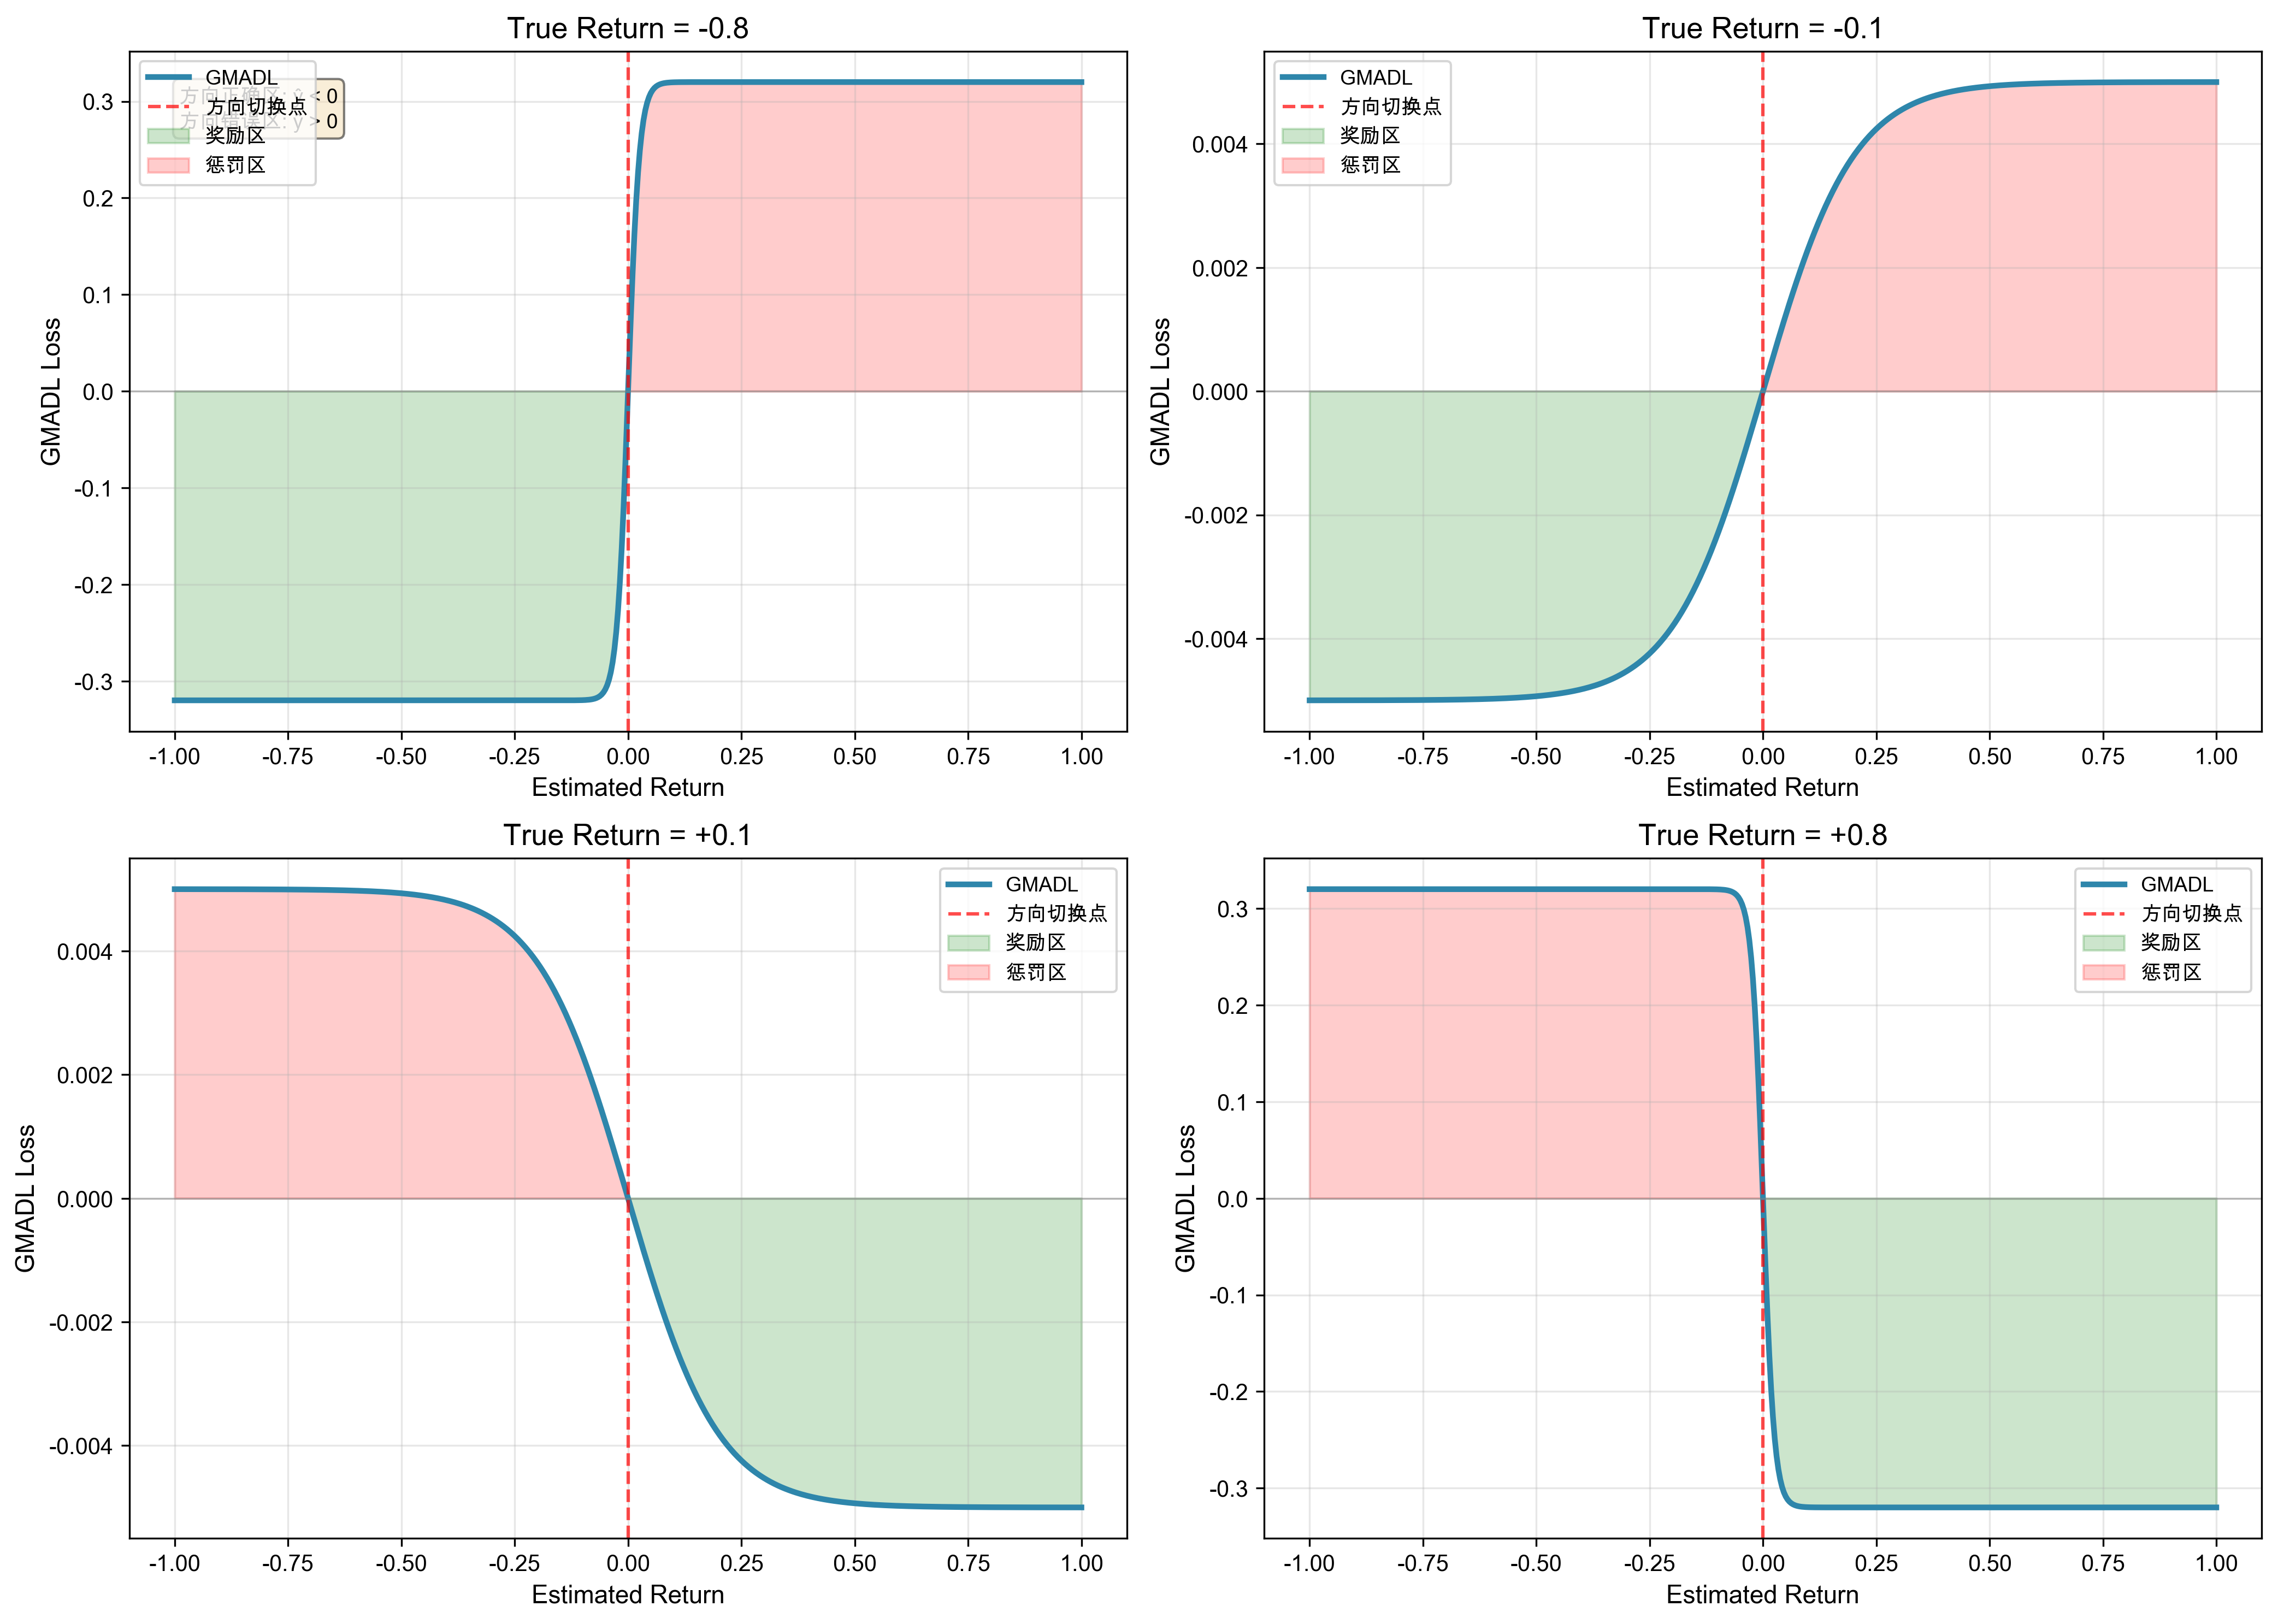
\includegraphics[width=0.95\textwidth]{gmadl_multiplot.png}
    \caption{GMADL Loss Function Behavior in Different Scenarios. The sigmoid transition provides a smooth gradient, identifying correct directions (negative loss/reward) versus wrong directions (positive loss/penalty).}
    \label{fig:gmadl_multi}
\end{figure}

\begin{figure}[H]
    \centering
    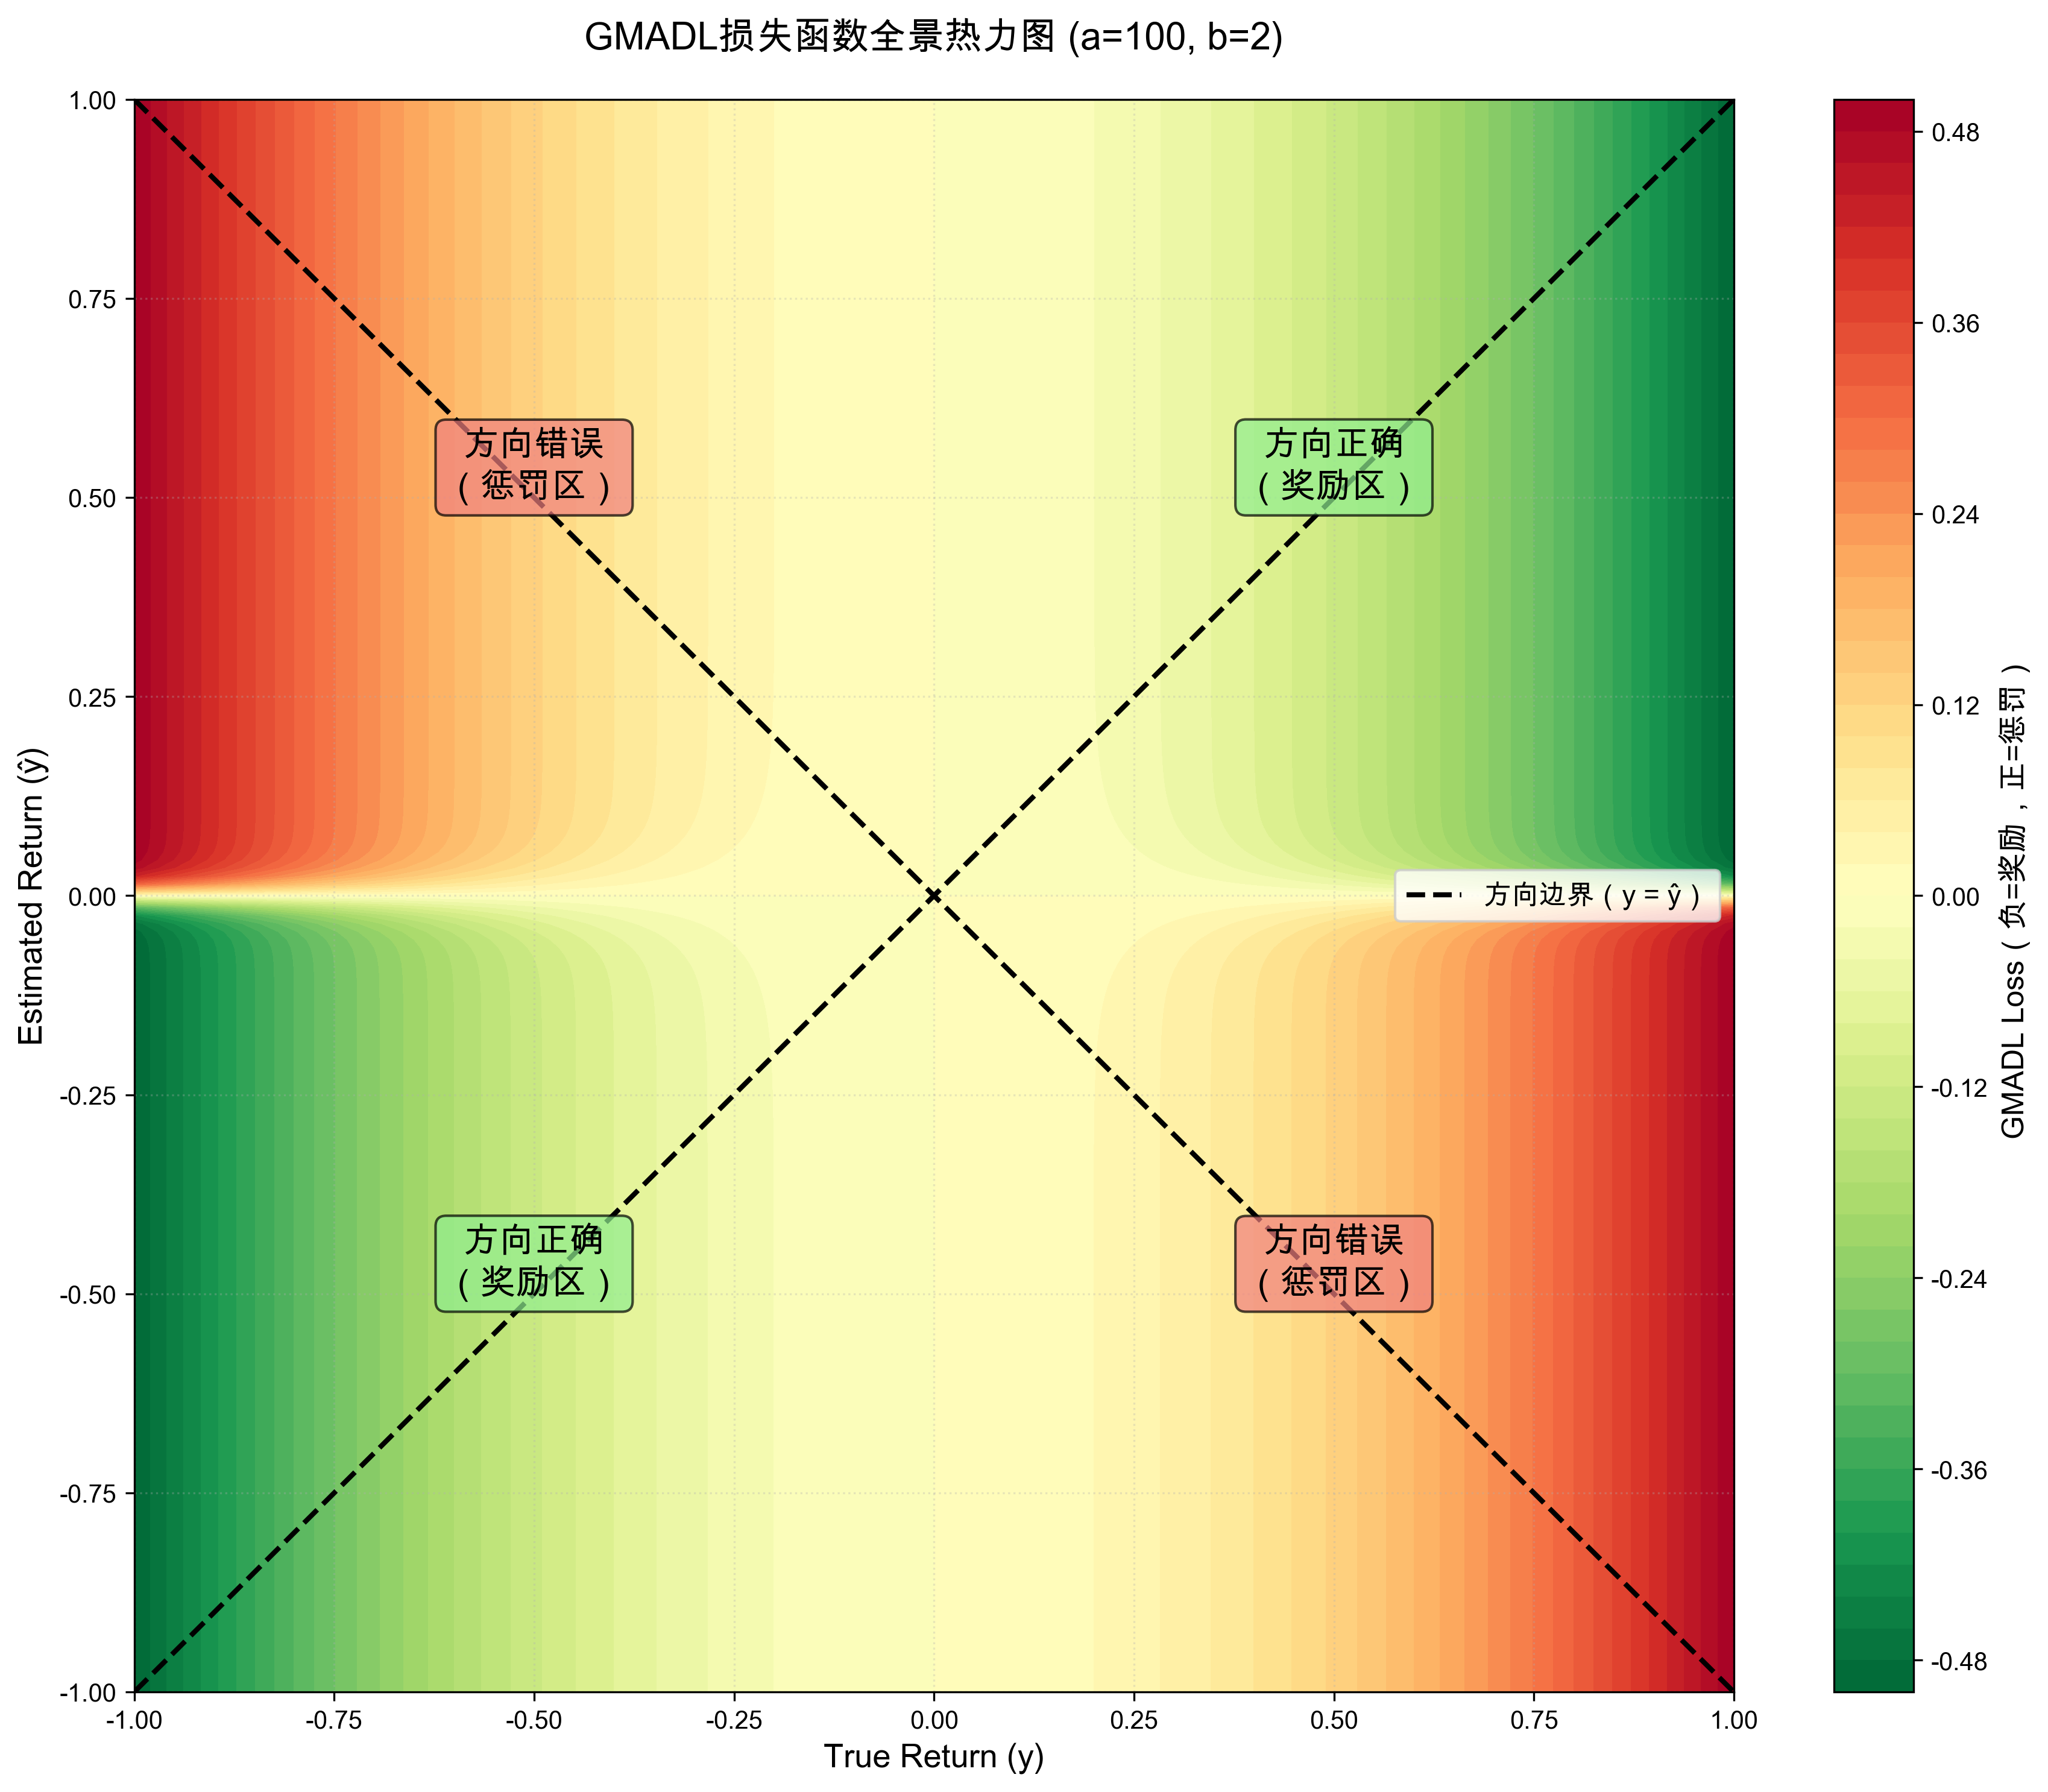
\includegraphics[width=0.8\textwidth]{gmadl_heatmap.png}
    \caption{GMADL Loss Function Heatmap ($a=100, b=2$). The diagonal boundary separates reward (green) and penalty (red) zones clearly.}
    \label{fig:gmadl_heat}
\end{figure}

\begin{figure}[H]
    \centering
    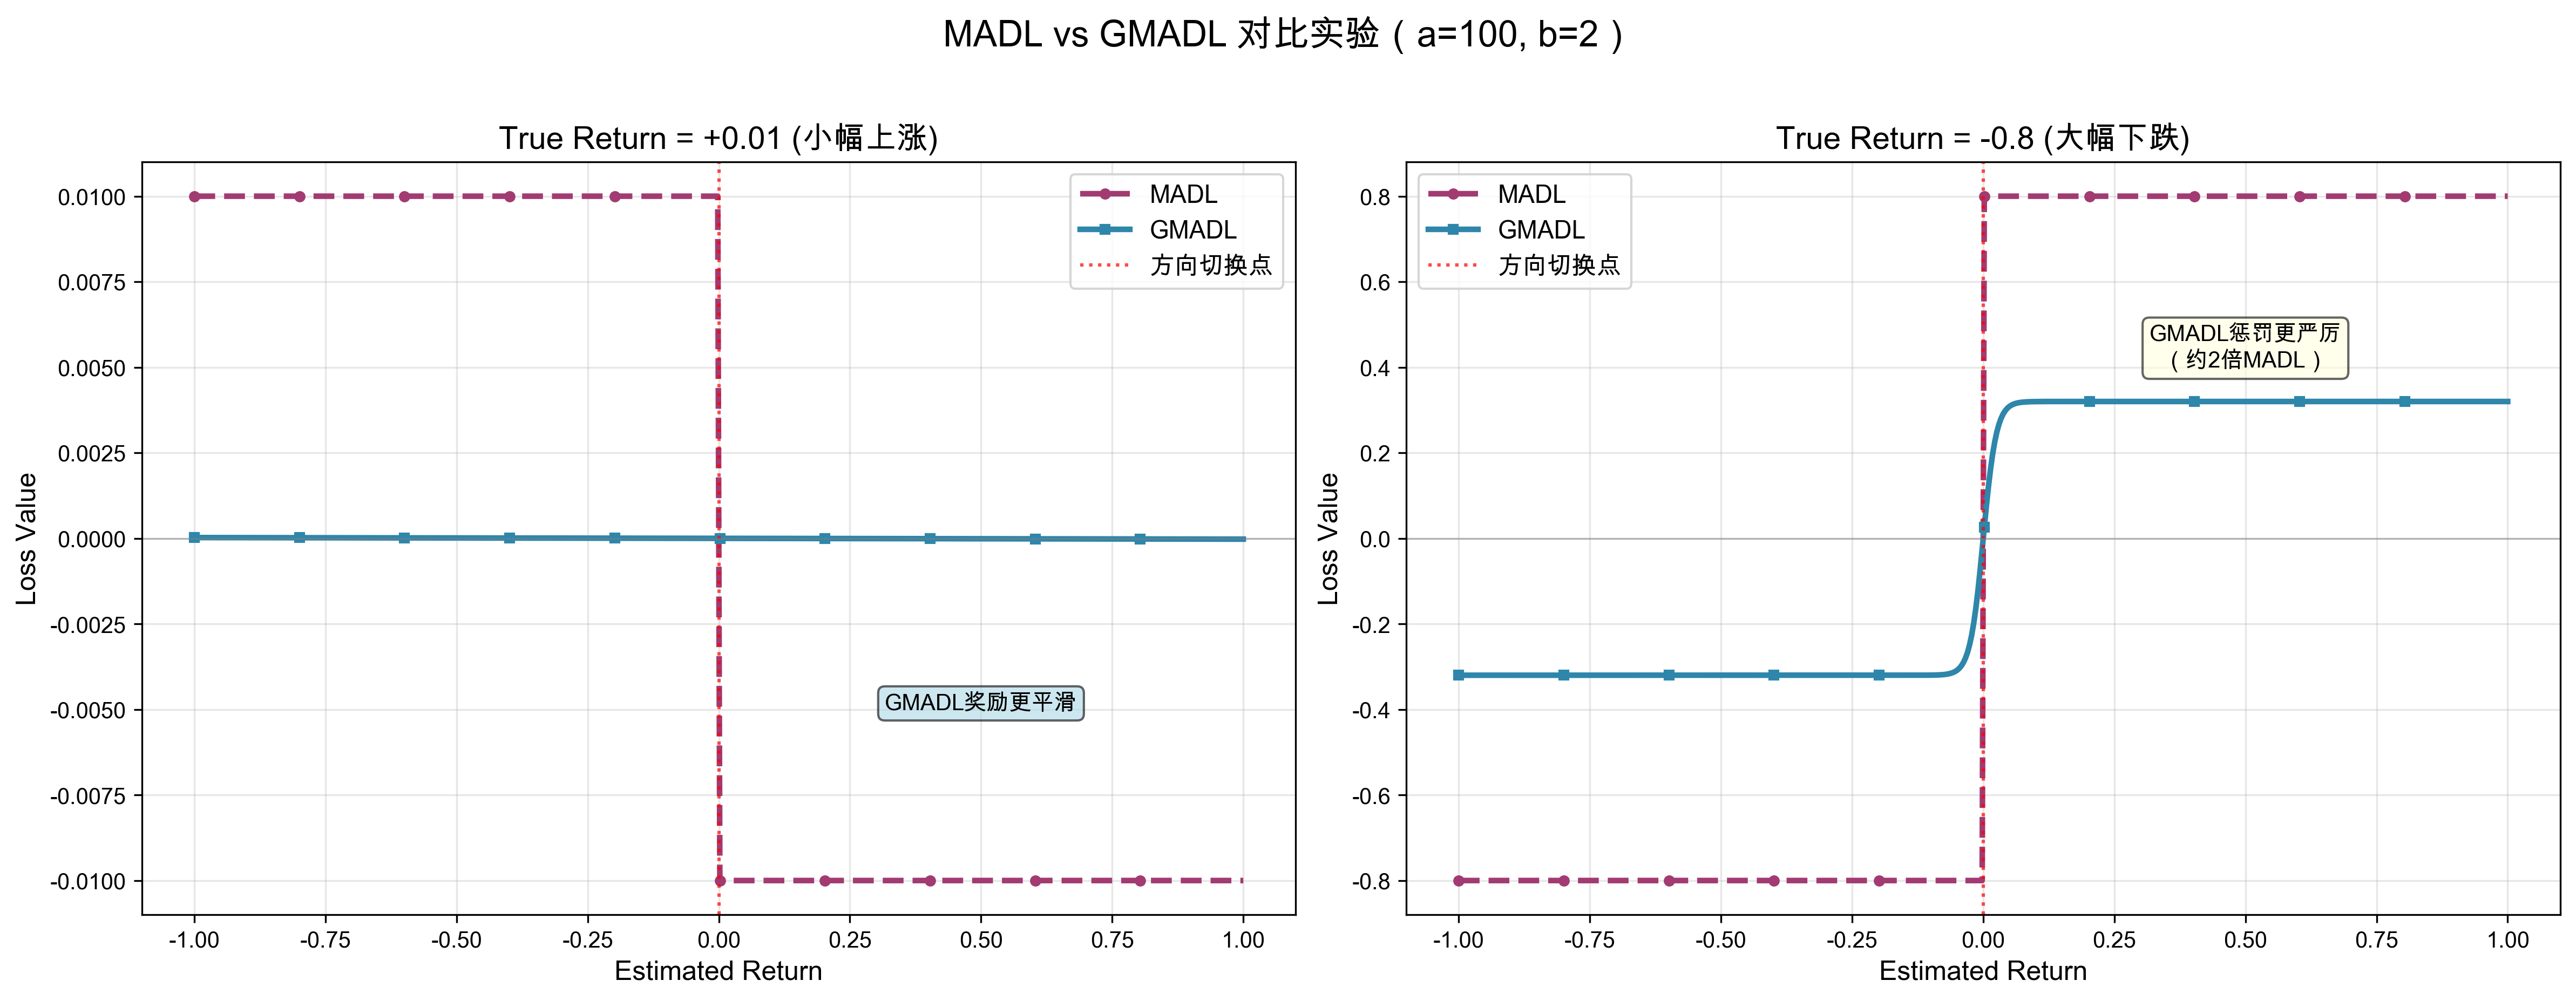
\includegraphics[width=1.0\textwidth]{madl_vs_gmadl_comparison.png}
    \caption{Comparison of MADL vs. GMADL. GMADL offers smoother derivatives but may lack incentives for precise magnitude prediction when direction is already correct.}
    \label{fig:madl_gmadl}
\end{figure}

\textbf{Key Findings \& Issues Identified:}
\begin{itemize}
    \item \textbf{Symmetry Issue:} Reward magnitude equals penalty magnitude. This fails to reflect the risk aversion principle ("avoiding loss $>$ chasing profit").
    \item \textbf{Weak Signal at Critical Points:} When $\hat{y} \to 0$, the sigmoid term approaches 0.5, resulting in a near-zero gradient, providing little learning signal.
    \item \textbf{Ignoring Precision:} Loss is correlated with $|y|$ and direction, but not explicitly with $|y - \hat{y}|$. A prediction of $+0.01$ and $+1.0$ yields similar rewards if the true return is $+0.1$, failing to incentivize precision.
\end{itemize}

\section{MSE vs. MedSE Portfolio Backtest Comparison}
I conducted backtests using three portfolio construction methods (P1, P2, P3) comparing MSE and MedSE loss functions.

\textbf{Portfolio Definitions:}
\begin{itemize}
    \item \textbf{P1 (Equal):} Long top 10\%, Short bottom 10\%, equal weights.
    \item \textbf{P2 (Signal Weighted):} Z-score normalization within Long/Short buckets. $z_{i,t} = \frac{\hat{y}_{i,t}-\mu_t}{\sigma_t}$. Weights are defined as $w_{i,t}^{raw} = \max(\pm z_{i,t}, 0)$.
    \item \textbf{P3 (Capped):} Adds a single stock weight cap (e.g., 10\%) to P2.
\end{itemize}

\textbf{Results:}
The results indicate significant differences. Table \ref{table:perf_comp} summarizes the performance metrics, and the subsequent figures illustrate the cumulative returns and risk profiles.

\begin{table}[H]
\centering
\caption{Strategy Performance Comparison (Jan-Jun 1995)}
\label{table:perf_comp}
\begin{tabular}{llrrr}
\toprule
\textbf{Strategy} & \textbf{Loss} & \textbf{Std} & \textbf{Sharpe} & \textbf{CumReturn} \\
\midrule
P1\_Equal & MSE & 0.0147 & 0.3730 & 0.9\% \\
P1\_Equal & MedSE & 0.0116 & 2.6773 & 5.48\% \\
P2\_SignalWeighted & MSE & 0.0288 & -1.4559 & -7.23\% \\
P2\_SignalWeighted & MedSE & 0.0282 & 3.2286 & 16.64\% \\
P3\_Cap & MSE & 0.0254 & -1.5668 & -6.86\% \\
P3\_Cap & MedSE & 0.0282 & 3.2286 & 16.64\% \\
\bottomrule
\end{tabular}
\end{table}

\begin{figure}[H]
    \centering
    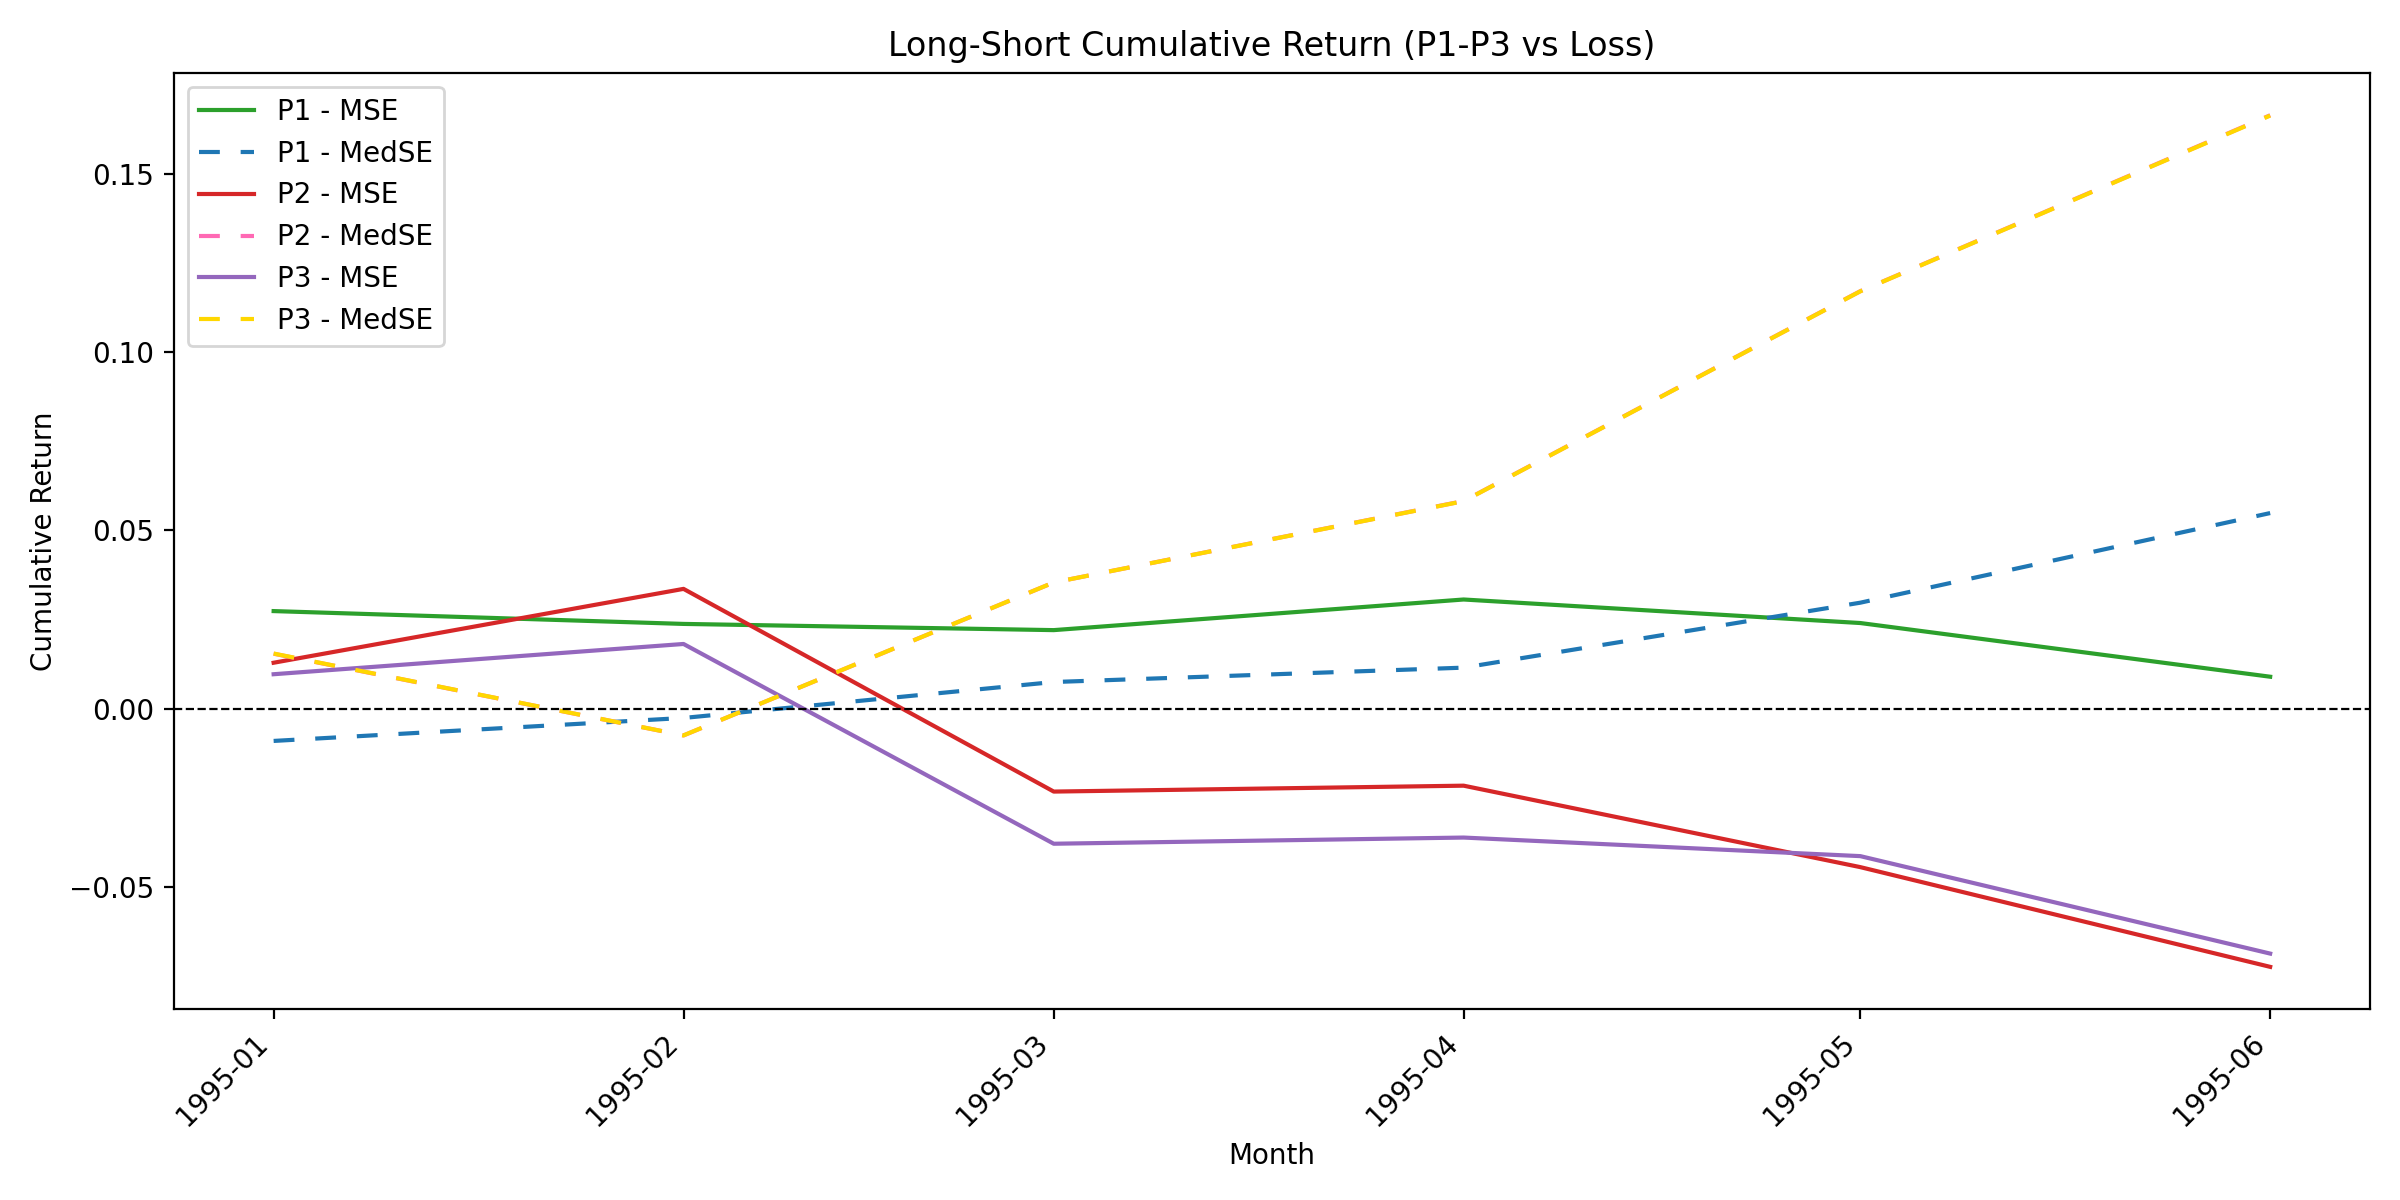
\includegraphics[width=0.9\textwidth]{strategy_loss_longshort.png}
    \caption{Long-Short Cumulative Return (P1-P3 vs Loss). MedSE (dashed lines) significantly outperforms MSE across all portfolio constructions.}
    \label{fig:cum_ret}
\end{figure}

\textbf{Detailed Risk and Return Analysis:}
The following panel compares the Standard Deviation and Sharpe Ratios across all strategies.

\begin{figure}[H]
    \centering
    % Top Row: Std and P1
    \begin{subfigure}[b]{0.48\textwidth}
        \centering
        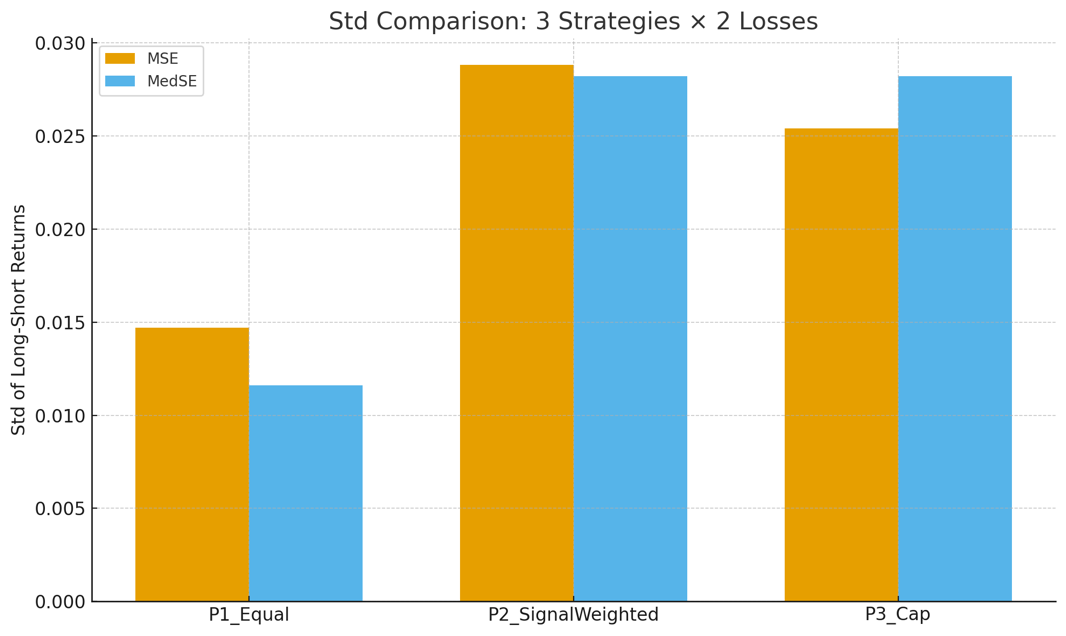
\includegraphics[width=\textwidth]{std.png}
        \caption{Standard Deviation}
    \end{subfigure}
    \hfill
    \begin{subfigure}[b]{0.48\textwidth}
        \centering
        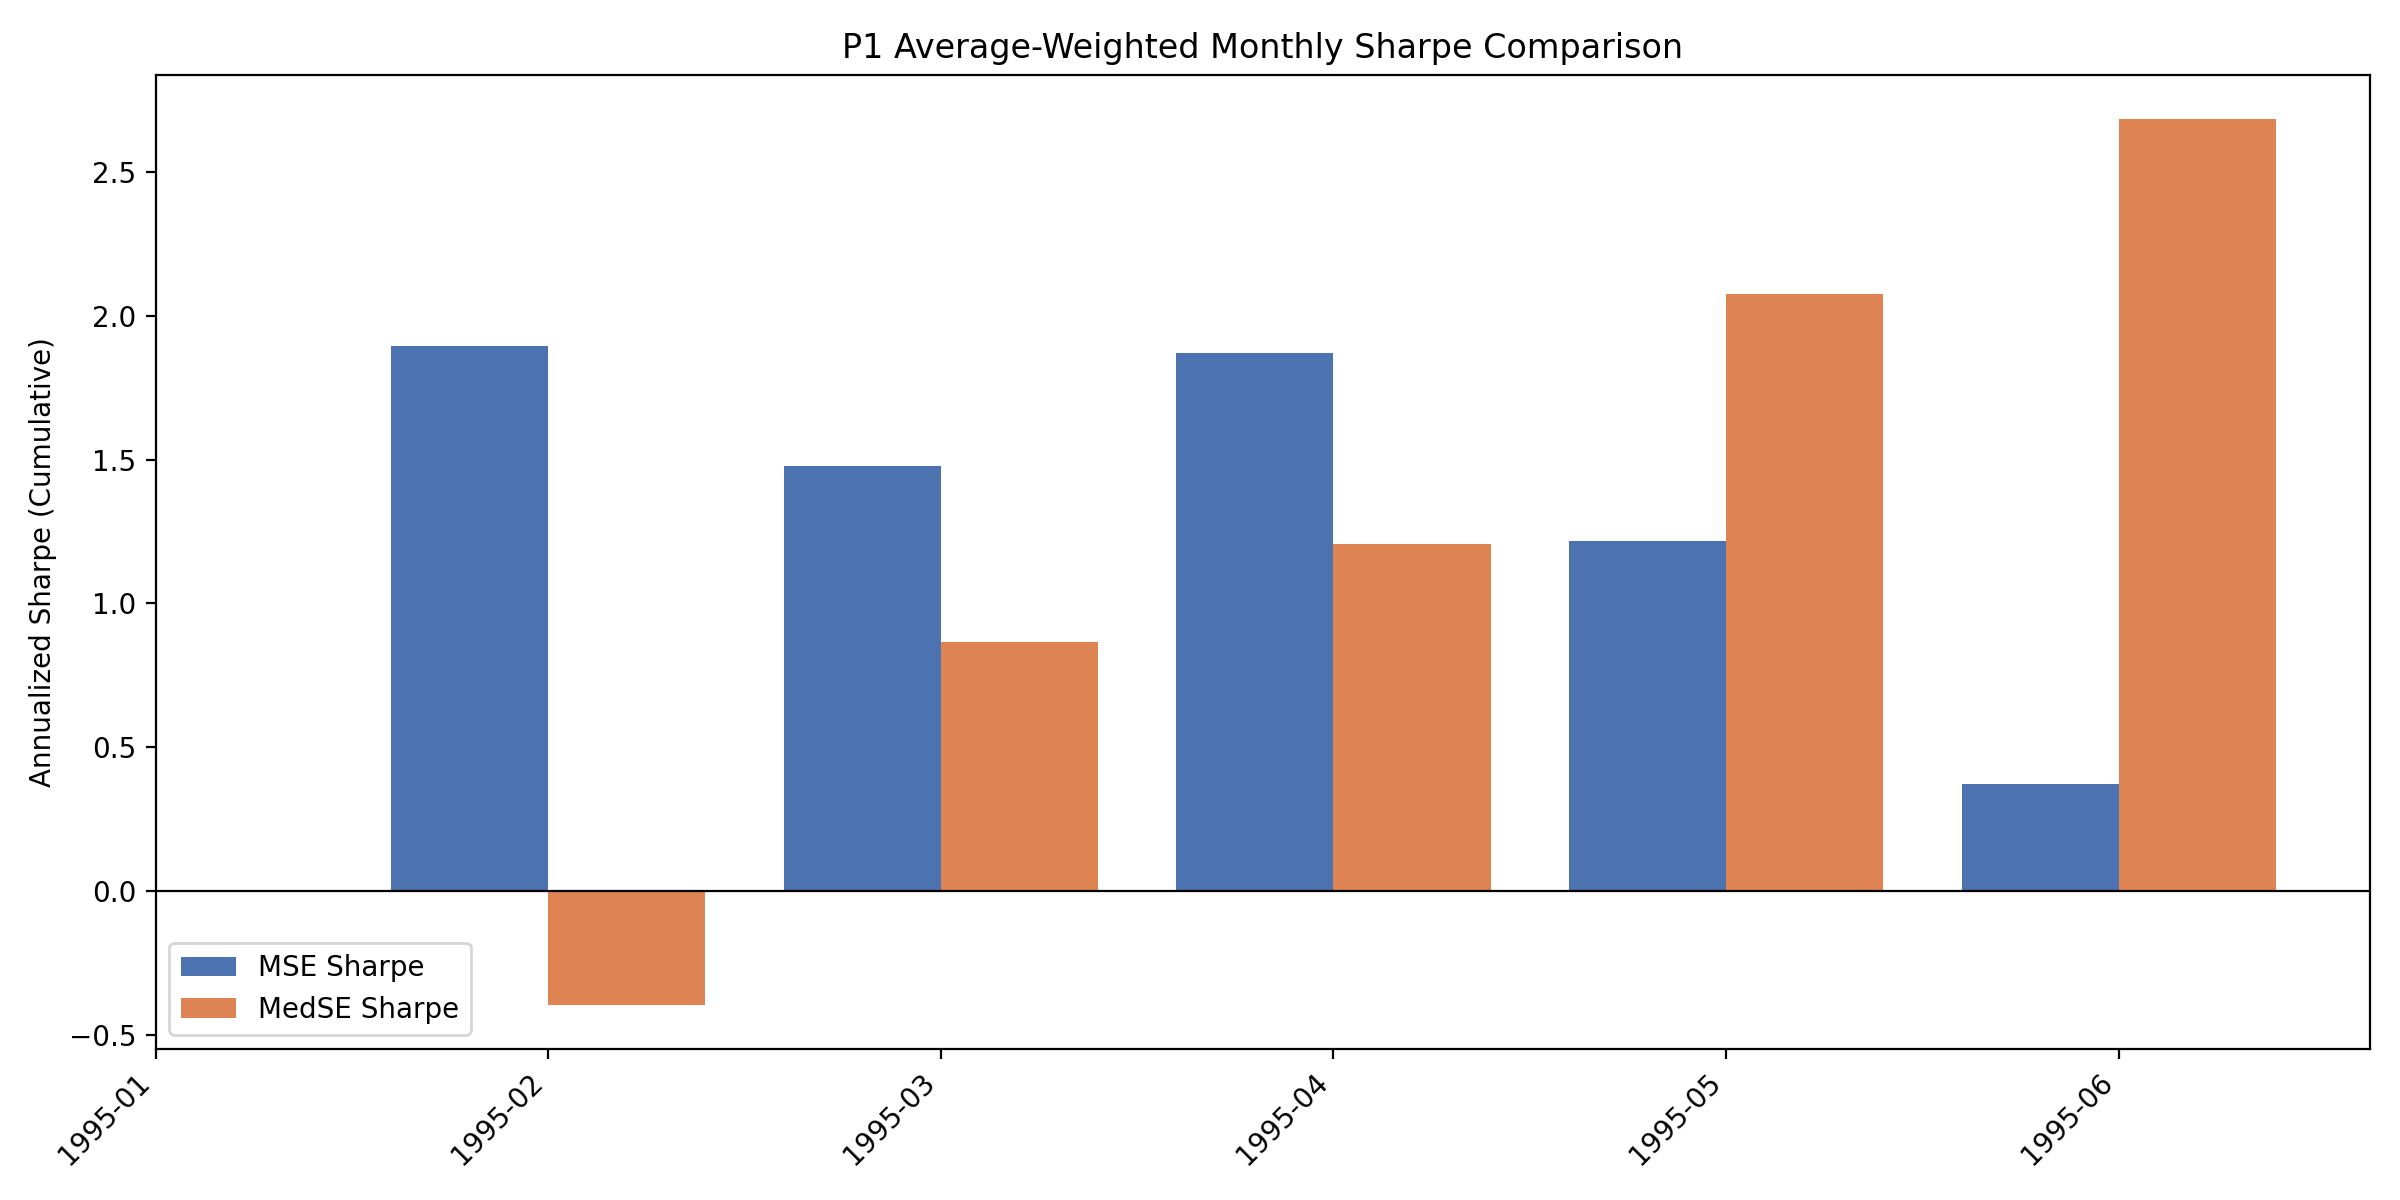
\includegraphics[width=\textwidth]{p1_weighted_sharpe.png}
        \caption{P1 (Equal) Sharpe}
    \end{subfigure}
    
    \vspace{0.5cm}
    
    % Bottom Row: P2 and P3
    \begin{subfigure}[b]{0.48\textwidth}
        \centering
        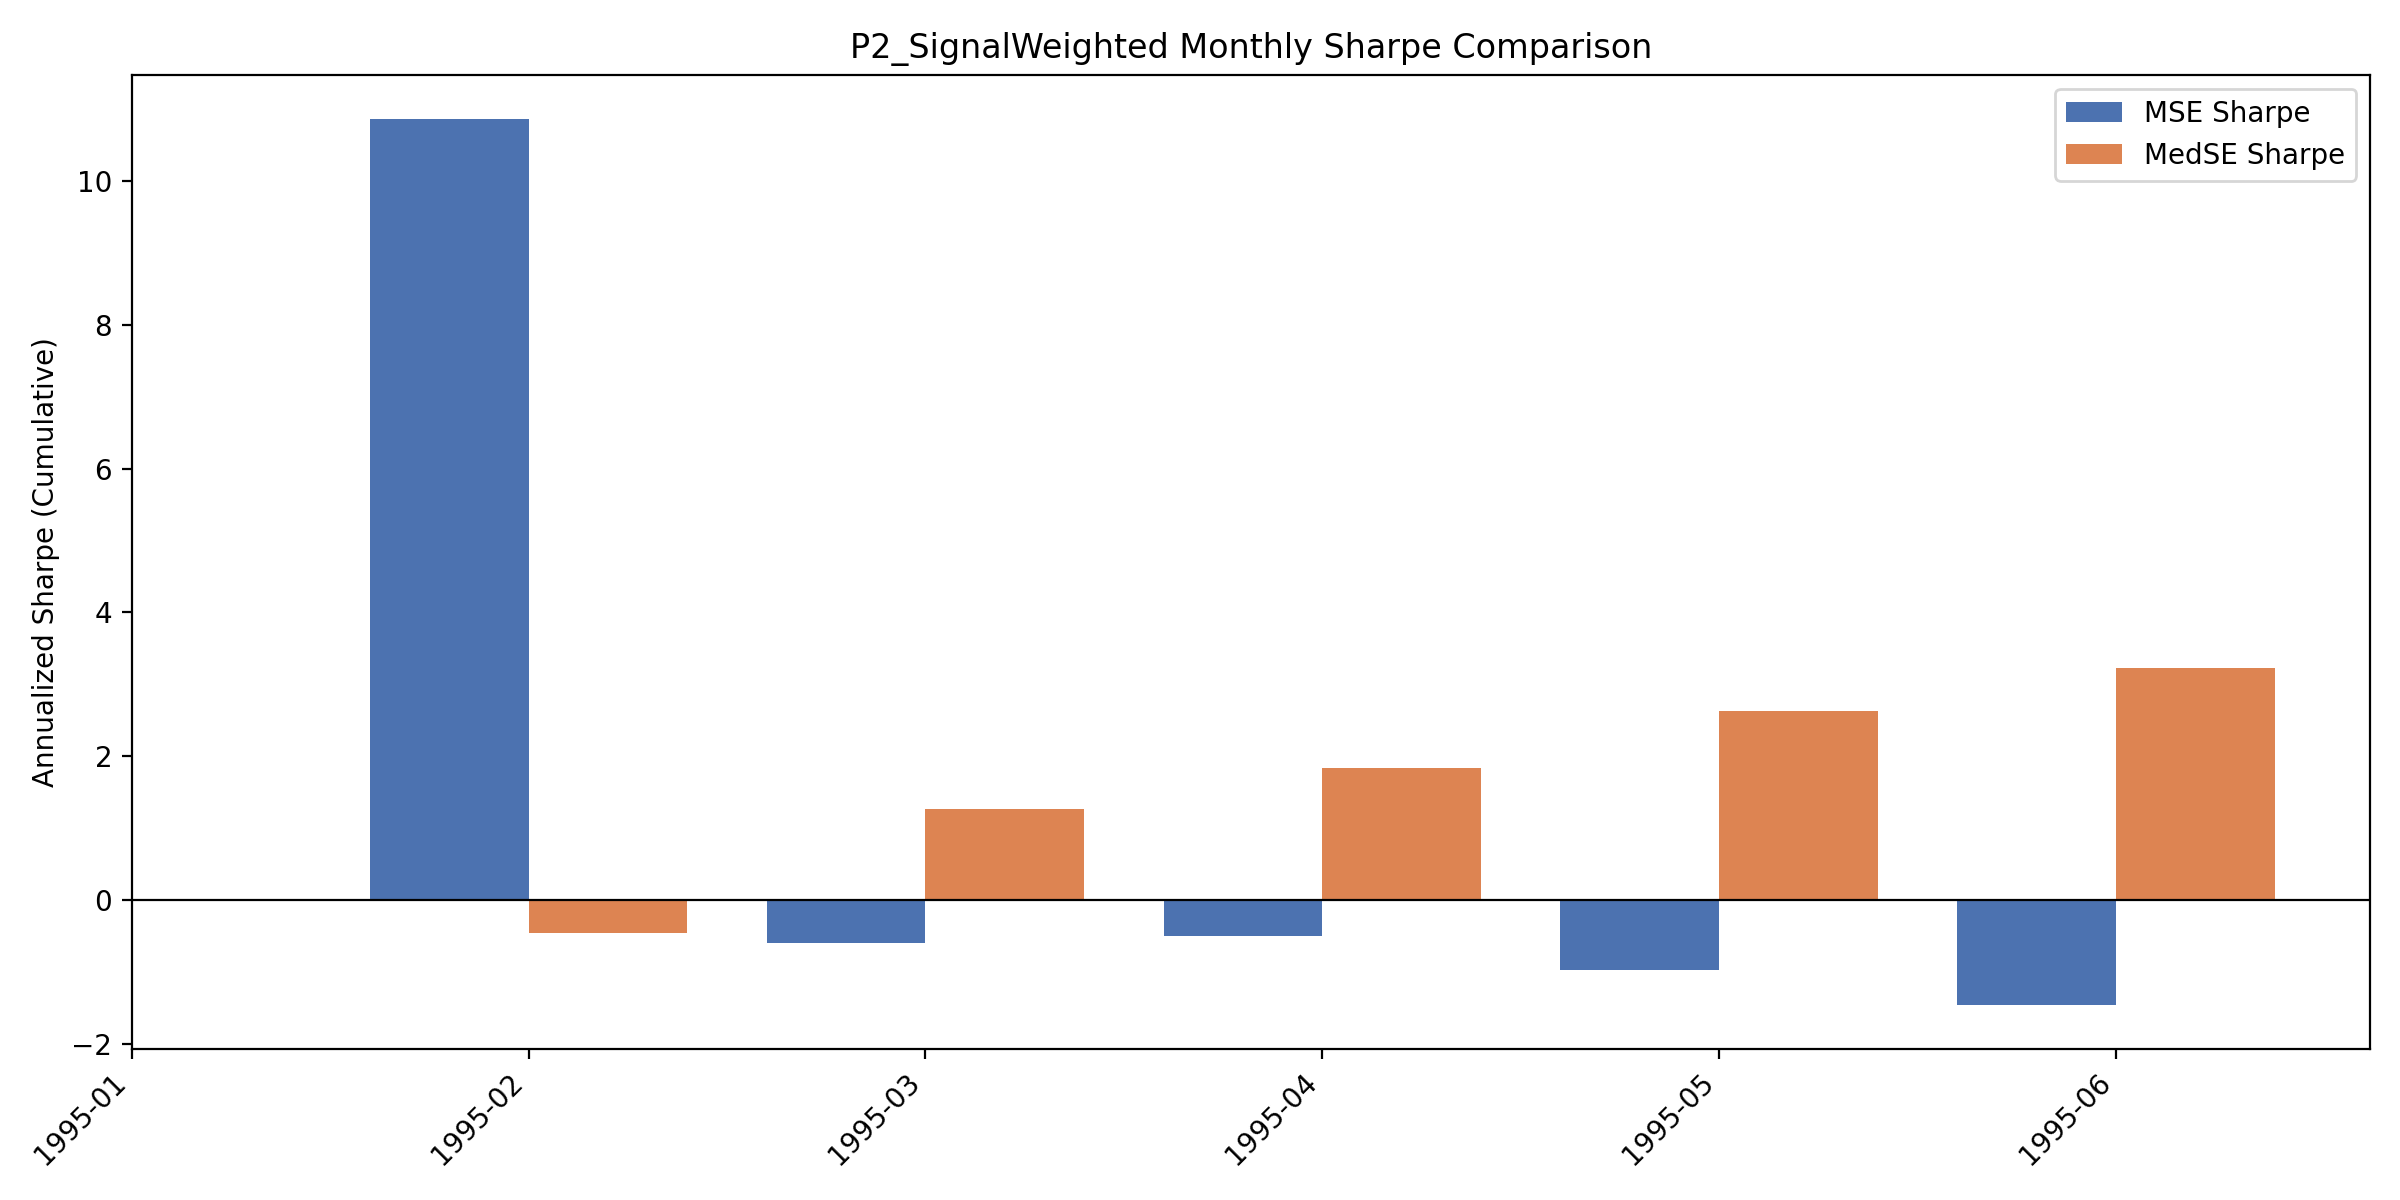
\includegraphics[width=\textwidth]{p2_signalweighted_sharpe.png}
        \caption{P2 (Signal Weighted) Sharpe}
    \end{subfigure}
    \hfill
    \begin{subfigure}[b]{0.48\textwidth}
        \centering
        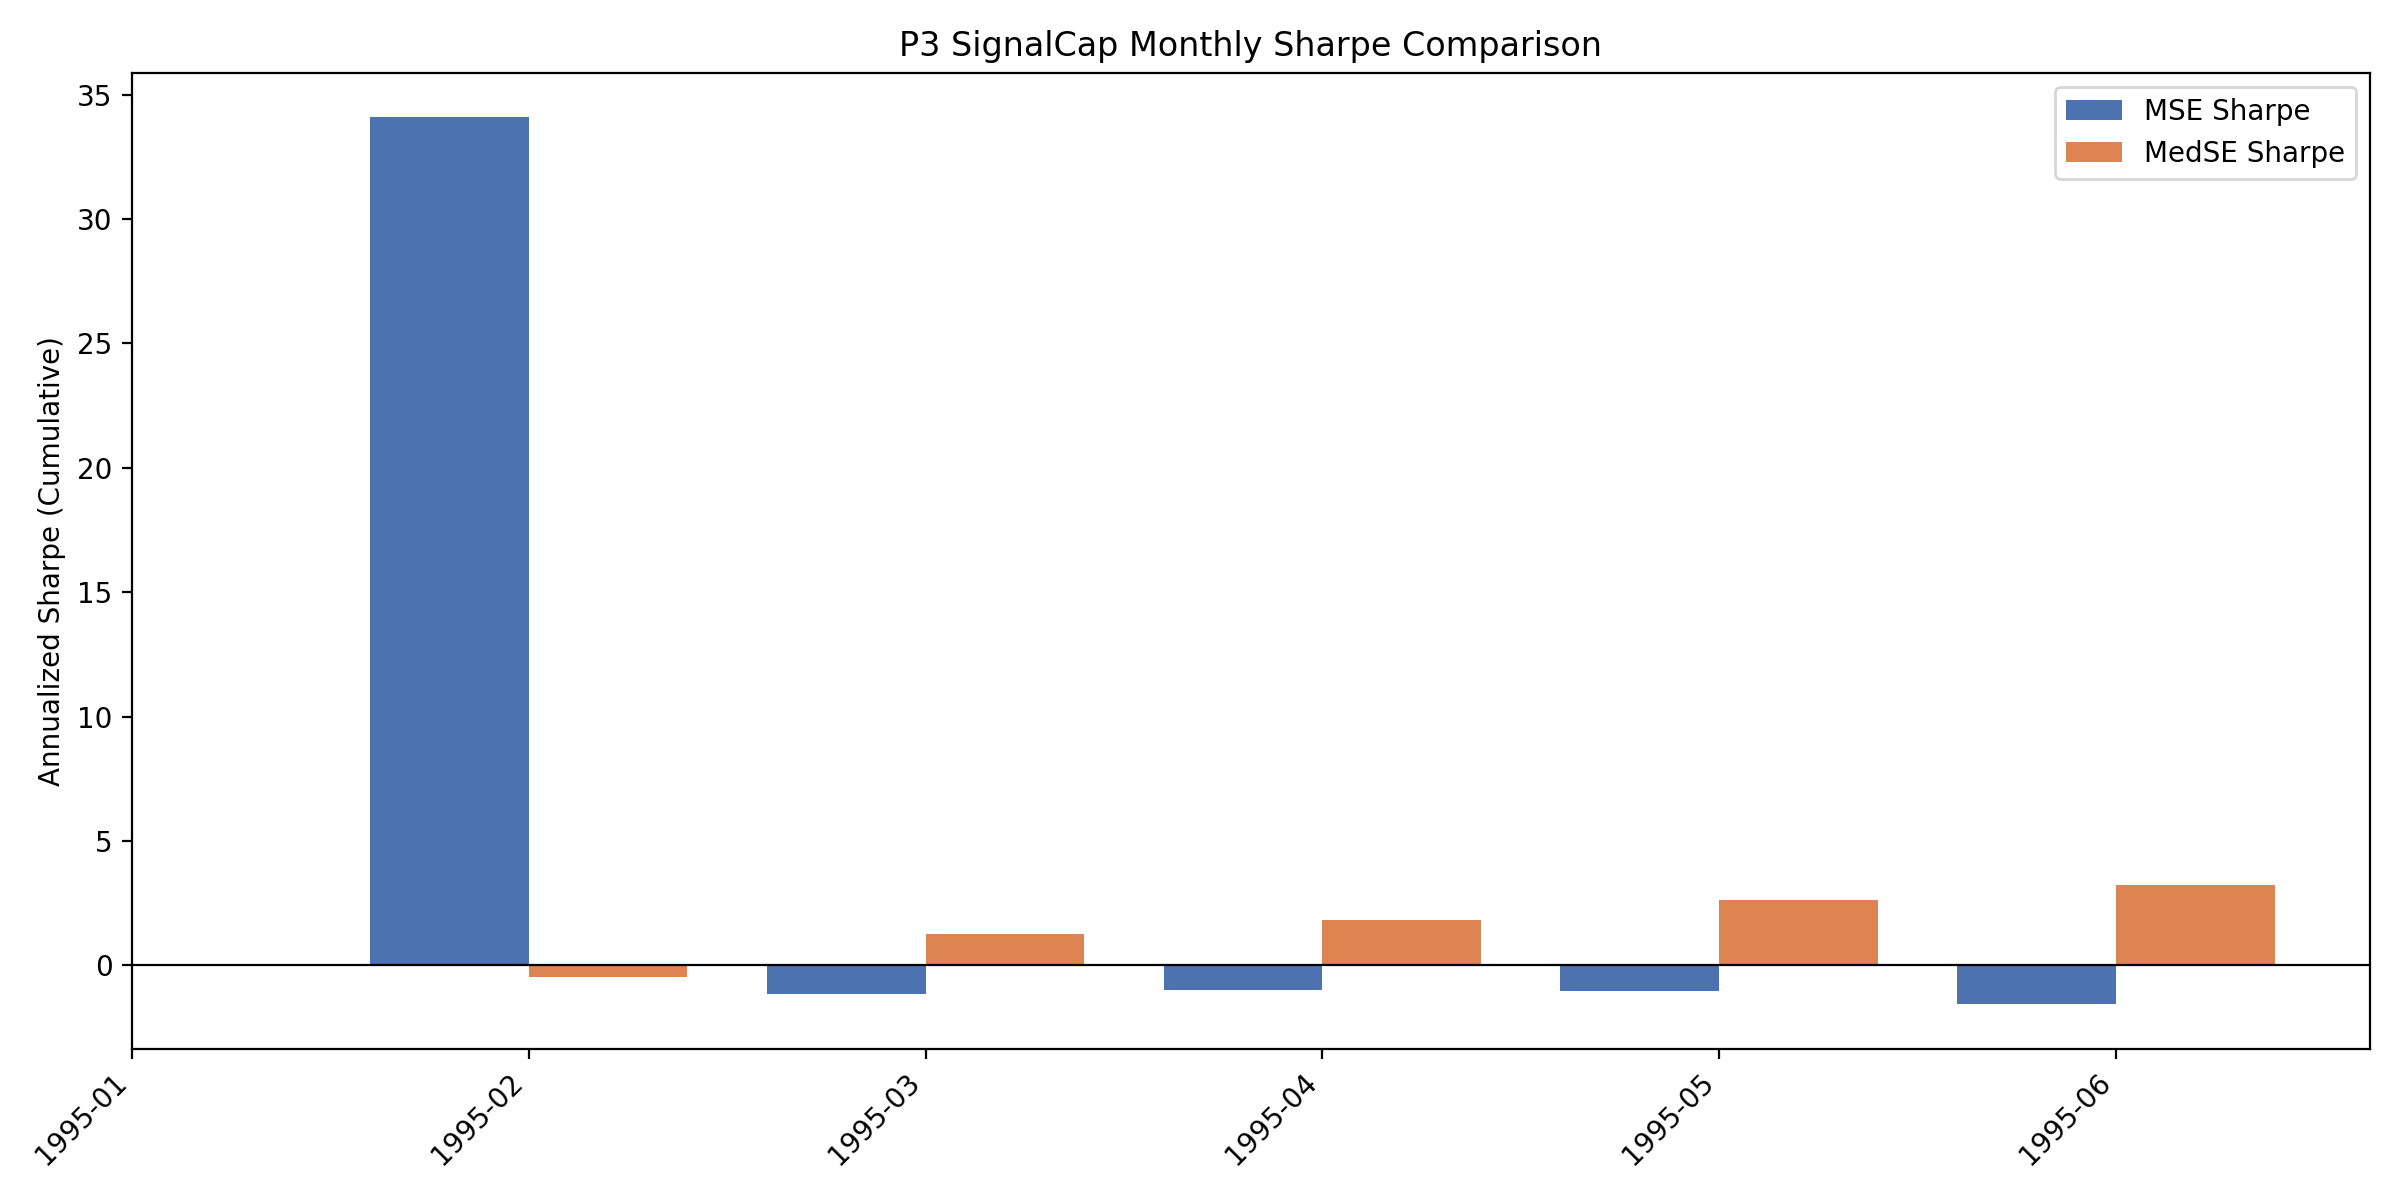
\includegraphics[width=\textwidth]{p3_signalCap_sharpe.png}
        \caption{P3 (Capped) Sharpe}
    \end{subfigure}
    
    \caption{Risk and Return Breakdown. (a) MedSE generally maintains comparable or lower volatility (Std). (b, c, d) Sharpe Ratios are significantly higher for MedSE across all portfolio weighting schemes, indicating superior risk-adjusted returns.}
    \label{fig:sharpe_panel}
\end{figure}

\textbf{Analysis:}
\begin{itemize}
    \item \textbf{Sharpe Ratio:} MedSE generates consistently positive and higher Sharpe ratios.
    \item \textbf{Risk:} In P1, MedSE has lower volatility (Std 0.0116 vs 0.0147). In P2/P3, volatilities are comparable, but MedSE achieves much higher returns (16.64\% vs -7.23\%), suggesting the performance boost is due to effective signal capture rather than excessive leverage.
\end{itemize}

% =========================================
% CHAPTER 5: KNOWLEDGE GAINED
% =========================================
\chapter{Knowledge Gained and Skills Required}

\section{Knowledge and Understanding Gained}
Through the comprehensive replication and analysis of the MADL and GMADL studies, I have developed a structured and rigorous approach to academic research.
\begin{enumerate}
    \item \textbf{Critical Literature Review \& Research Lifecycle:}
    I have learned to critically deconstruct academic literature, identifying the gap between theoretical loss functions and their practical financial implications. This process clarified the end-to-end research workflow, from initial hypothesis formulation to rigorous empirical validation, allowing me to understand how academic theories translate into actionable trading strategies.
    
    \item \textbf{Technical Proficiency in the Machine Learning Pipeline:}
    I have gained independence in executing the complete machine learning pipeline. Specifically, I mastered independent feature engineering and acquired a profound understanding of essential protocols such as Grid Search for hyperparameter optimization. Furthermore, I now clearly distinguish the methodological differences and applications between static train-test splits and rolling-window backtesting, which is crucial for time-series financial data.
    
    \item \textbf{Integration of Mathematical Theory and Trading Intuition:}
    Leveraging my mathematical background and intuition for trading mechanics, I successfully designed and tested novel portfolio construction methods—specifically the signal-weighted and capped approaches. The positive empirical feedback from these designs has validated the effectiveness of integrating domain-specific financial logic into quantitative model design.
\end{enumerate}

\section{New Skills Required}
Through the reproduction of GMADL and the initial experiments, I have identified several key technical areas that require further mastery:
\begin{itemize}
    \item \textbf{Custom Gradient Implementation:} Using PyTorch's `autograd` and `gradcheck` to handle numerical stability in custom loss functions (e.g., handling Sigmoid saturation).
    \item \textbf{High-Performance Data Processing:} Utilizing Dask and HDF5 for rolling window calculations to reduce feature engineering time.
    \item \textbf{Bayesian Optimization:} Employing Optuna for efficient hyperparameter tuning in high-dimensional spaces.
    \item \textbf{Theoretical Foundations:} Understanding M-estimators and Robust Statistics (Huber, 1964) to justify the robustness of proposed loss functions.
\end{itemize}

% =========================================
% CHAPTER 6: MAJOR CHALLENGES
% =========================================
\chapter{Major Challenges}
\begin{enumerate}
    \item \textbf{Numerical Stability:} The proposed directional penalty involves Sigmoid approximations and max-clipping. When $y \approx 0$, gradients may vanish. Solutions include gradient clipping and smooth approximations.
    \item \textbf{Hyperparameter Complexity:} The search space (penalty weights, smoothing factors) is large. I plan to use hierarchical Bayesian optimization.
    \item \textbf{Computational Resources:} Rolling backtests require training $\sim 12,000$ models (60 rebalances $\times$ configs). This requires optimized code and potentially 15-20 days of GPU time.
    \item \textbf{Time Management:} Balancing coursework (Time Series Analysis, Strategic Management) with this research. I have established a strict schedule (dedicated project blocks on Mon/Wed/Fri).
\end{enumerate}

% =========================================
% CHAPTER 7: PLAN FOR SEMESTER 2
% =========================================
\chapter{Plan and Timeline for Semester 2}

\section{Research Plan Overview}
The focus for Semester 2 is to design and implement two customized asymmetric loss functions:

\textbf{Method 1: Non-negative Directional Penalty Loss} \\
Addresses the "negative reward" issue in GMADL. It converts the mechanism into a standard penalty framework: applying a penalty proportional to return magnitude only when the direction is wrong. This serves as a robust baseline.

\textbf{Method 2: Hybrid Ranking-Aware Loss} \\
Incorporates Learning-to-Rank (LTR) mechanisms. Since portfolio construction is essentially a ranking problem (identifying top/bottom deciles), this method introduces a pairwise ranking loss alongside the directional penalty to directly learn the relative order of assets.

\section{Timeline}
\begin{itemize}
    \item \textbf{Weeks 1-4 (Foundation):} Implement Method 1 (Directional Penalty). Smooth the function for differentiability. Initial training on Feature Set X.
    \item \textbf{Weeks 4-8 (Benchmark Experiments):} Apply Method 1 to all feature sets. Compare against NN-Mean, NN-Median. Execute rolling backtests (5-year train, 6-month predict). Compute Out-of-Sample RMSE and Sharpe Ratios. Start implementation of Method 2 (Ranking Loss).
    \item \textbf{Weeks 9-10 (Writing \& Integration):} Finalize theoretical proofs (convexity, gradient properties). Compile all empirical results. Write the final thesis chapters (Introduction, Literature Review, Methodology, Results).
\end{itemize}

% =========================================
% BIBLIOGRAPHY
% =========================================
\cleardoublepage


\begin{thebibliography}{99}

\bibitem{lopez2013look}
Lopez de Prado, M. (2013). What to look for in a backtest. \textit{Available at SSRN}.

\bibitem{bailey2017probability}
Bailey, D.H., Borwein, J., Lopez de Prado, M., \& Zhu, Q.J. (2017). The probability of backtest overfitting. \textit{Journal of Computational Finance}, 20(4), 39-69.

\bibitem{di2016artificial}
Di Persio, L., \& Honchar, O. (2016). Artificial neural networks architectures for stock price prediction: Comparisons and applications. \textit{International Journal of Circuits, Systems and Signal Processing}, 10, 403-413.

\bibitem{yang2019deep}
Yang, J., Li, Y., Chen, X., Cao, J., \& Jiang, K. (2019). Deep learning for stock selection based on high frequency price-volume data. \textit{arXiv preprint arXiv:1911.02502}.

\bibitem{wiecki2016all}
Wiecki, T., Campbell, A., Lent, J., \& Stauth, J. (2016). All that glitters is not gold: Comparing backtest and out-of-sample performance on a large cohort of trading algorithms. \textit{Journal of Investing}, 25(3), 69-80.

\bibitem{topcu2020impact}
Topcu, M., \& Gulal, O.S. (2020). The impact of COVID-19 on emerging stock markets. \textit{Finance Research Letters}, 36, 101691.

\bibitem{michankow2024mean}
Michańków, J., Sakowski, P., \& Ślepaczuk, R. (2024b). Mean absolute directional loss as a new loss function for machine learning problems in algorithmic investment strategies. \textit{Journal of Computational Science}, 81, 102375.

\bibitem{michankow2024generalized}
Michańków, J., Sakowski, P., \& Ślepaczuk, R. (2024a). Generalized mean absolute directional loss as a solution to overfitting and high transaction costs. \textit{arXiv preprint arXiv:2412.18405}.

\bibitem{gu2020empirical}
Gu, S., Kelly, B., \& Xiu, D. (2020). Empirical asset pricing via machine learning. \textit{Review of Financial Studies}, 33(5), 2223-2273.

\end{thebibliography}

\end{document}